\chapter{The wires}

To simplify the analysis of the wires parasitics effects we introduce 3 simple assumption;\\
\vspace{2mm}
\tab $\rightarrow$ Inductance can be neglected if the wire resistance is large or if the rise/fall time of the input signal is large.\\
\vspace{2mm}
\tab $\rightarrow$ When the wire is short and when the equivalent resistance of the driver is large, the wire resistance can be serenely neglected.\\
\vspace{2mm}
\tab $\rightarrow$ When the separation between nearby wires is large or when the wires run in parallel for a short distance, the inter-wires capacitance can be neglected.\\


%------------------------------------------------------------------------%
%------------------------------------------------------------------------%
\section{Capacitance}

\centering
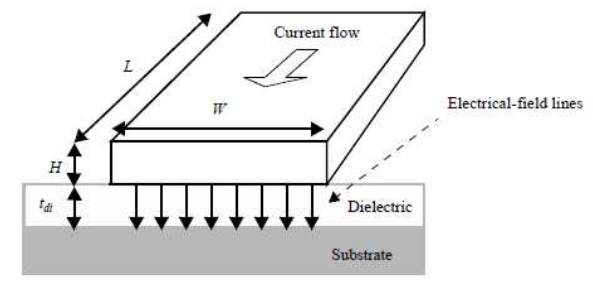
\includegraphics[width=0.5\textwidth]{C5_1.png}\\
\raggedright

We divide the overall capacitance of a wire in 2 main contribution; parallel plate capacitance and fringing capacitance.\\
In the ideal case where the parameter $W/t_{di}$ is very large the fringing capacitance contribution can be neglected but since in our reference technology we can have $W/H>1$ the fringing or border capacitance is the dominant contribution.\\
\vspace{5mm}

For our reference technology process the following table is given reporting the parallel-plate and the fringing capacitance contributions for a wire in a certain layer with respect to another wire in another layer.\\
The parallel-plate capacitance is reported in the white rows expressed in $aF/\mu m^2$ of overlapping area, while the shaded rows report the fringing capacitance contribution in $aF/\mu m$ of perimeter (that is quite always $\simeq 2L$).\\

\centering
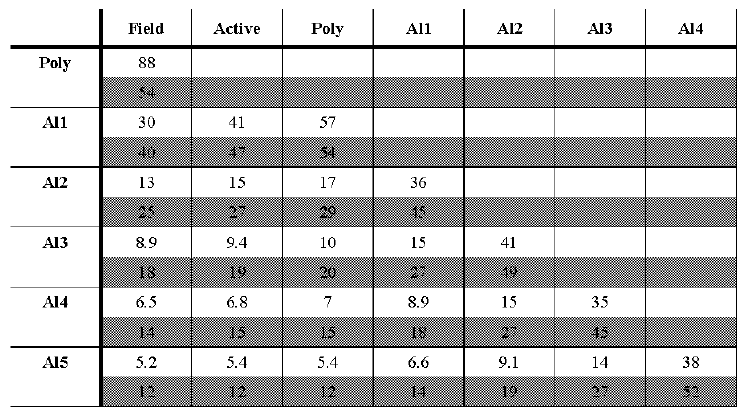
\includegraphics[width=0.8  \textwidth]{C5_2.png}\\
\raggedright
When using this table we have always to look what tipe of metal is our wire (rows) and in what material is made the ground plane or the other wire (columns) in order to get the correct values.\\

\vspace{3mm}
To evaluate che capacitance of 2 nearby wires implemented in the same layer at minimum distance we get the following table with the vales of the capacitances for unit lenght expressed in $aF/\mu m$ \\
\vspace{3mm}

\centering
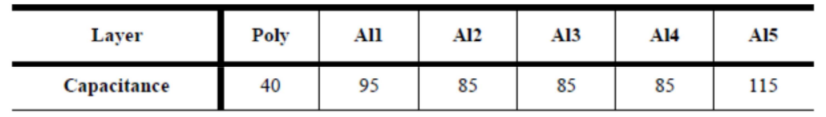
\includegraphics[width=0.8\textwidth]{C5_3.png}\\
\raggedright


%------------------------------------------------------------------------%
%------------------------------------------------------------------------%
\section{Resistance}

Resistance of a wire can be assested as
\begin{equation}
R=\rho \frac{L}{WH}=R_{sh}\frac{L}{W}
\end{equation} 
where the last part represent the resistance per square multiplied by the number of squares.\\
\vspace{5mm}
At very high frequency, the resistance tends to increase due to the skin effect. In practice the current tends to flow in the peripheral part of the wire. Considering a wire with a width W and a height H, the current flows almost entirely in a peripheral section characterized by a depth
\begin{equation}
\sigma=\sqrt{\frac{\rho}{\pi f \mu }}
\end{equation}
if the wire is smaller than the skin effect at a given frequency there are no difference in the resistance. It's an effect that affects only wide wires.\\


%------------------------------------------------------------------------%
%------------------------------------------------------------------------%
\section{Models for wires}



\subsection{Lumped C model}
Since the resistance of the wire is much smaller wrt the driving resitance we can model the wire with only it's capacitance.

\centering
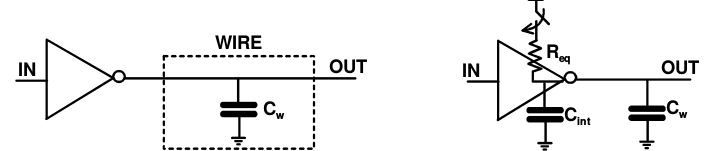
\includegraphics[width=0.5\textwidth]{C5_4.png}\\
\raggedright

The wire capacitance has to be added to the intrinsic capacitance of the inverter in order to correctly estimate the propagation delay that in this case is 
\begin{equation}
\tau=\ln(2)R_{eq}(C_{int}+C_w)
\end{equation}



\subsection{Lumped RC model}
When the resistance is no more negligible a first odrer approximation is to model the wire as it's single equivalent resistace and capacitance 

\centering
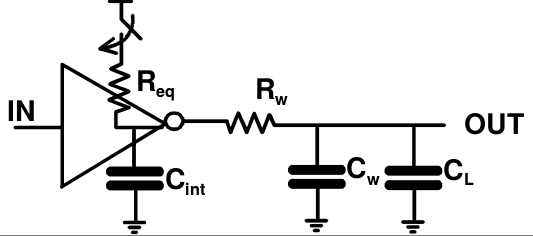
\includegraphics[width=0.35\textwidth]{C5_5.png}\\
\raggedright

To estimate the overall propagation we can model the circuit as follows and use the Elmore theorem

\centering
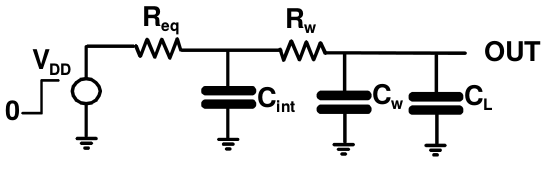
\includegraphics[width=0.35\textwidth]{C5_6.png}\\
\raggedright


\centering

\fbox{\begin{minipage}{40em}
\centering
{\bf Elmore theorem}\\
\raggedright
With a network that has a single input node ,all capacitance between a node and ground and no resistive loops we can assest the propagation delay of the line as calculating for every capacitance C of the network the so called shared-path resistance. This resistance represents the resistance shared between the path from the source of the signal and the output and the path form the source to the capacitance.\\

\centering
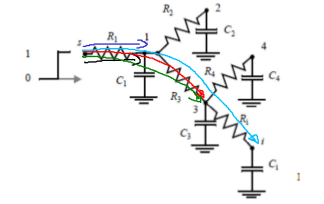
\includegraphics[width=0.35\textwidth]{C5_7.png}\\
\raggedright

\begin{equation}
\tau=C_1R_1+C_2R_1+C_3(R_1+R_3)+C_4(R_1+R_3)+C_j(R_1+R_2+R_j)
\end{equation}

\end{minipage}}

\raggedright
\vspace{5mm}

This is an approximation that brings us to an overestimation of the propagation delay (factor 2) beacuse we are supposing all parasitic terms concentrated in one point and not distributed over a line.\\

\subsection{Distributed model}
With the distributed model we divide the wire into lot of wires of length $\Delta L$ with $\Delta L \rightarrow 0$.\\

\centering
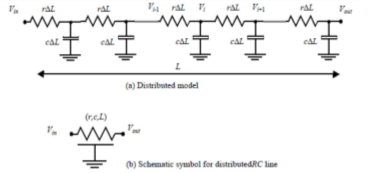
\includegraphics[width=0.5\textwidth]{C5_8.png}\\
\raggedright

In this way through the resoluton of a differential equation for the voltage over the line we get that the delay of the wire is 
\begin{equation}
\tau_w\simeq \ln(2)\frac{R_wC_w}{2}
\end{equation}
That is the correct value wrt the lumped RC model.\\

To correctly take into account the effects of the distribution we will use the following 2 models that give us both the same result of the distributed model

\centering
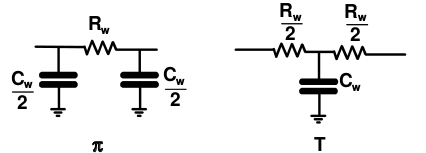
\includegraphics[width=0.35\textwidth]{C5_9.png}\\
\raggedright


\section{Buffering of a line}

If the time constant of a line it's the dominant contribution for delay in our digital circuit it's worth in order to get a faster respnce to cut the wire in N pieces adding buffer in the middle.\\
This is convenient if
\begin{equation}
L\ge\sqrt{\frac{16C_{int}R_{eq}}{cr}}
\end{equation}
where $C_{int},R_{eq}$ are parameters of the driving circuit and c,r are the specific resistance ($\Omega/m$) and capacitance ($F/m$) of the wire.
The optimum number of division N (and so the number of inverter to be added N-1) is
\begin{equation}
N=\sqrt{\frac{R_wC_w}{4C_{int}R_{eq}}}=L\sqrt{\frac{rc}{4C_{int}R_{eq}}}
\end{equation}
And the contribution to $\tau_p$ of the wire ($R_wC_w/2$) decreases by a factor N.\\
The propagation delay of an optimized line that is broken in N peices is 
\begin{equation}
\tau_p=\ln(2) N \left(R_{eq}C_{int}+(R_{eq}+\frac{R_w}{2N})\frac{C_w}{N}+(R_{eq}+\frac{R_w}{N})C_{int}\right)
\end{equation}
In this expression we supposed inverters with the same size and $\gamma=1$.\\
This optimization of the line it's indipendent form the size of the stage present in the circuit.\\

\section{Inductance}

Parasitic inductances can be neglected if the time of flight of the signal is much less than the minimum propagation delay of the circuit. With a line of length L and the maximum propagation delay of $\tau_{max}$ this translates as 
\begin{equation}
t_{flight}=\frac{L}{\frac{c}{\sqrt{\mu \varepsilon}}}\ \  << \ \ \tau_{max}     
\end{equation}
where tipically $\varepsilon=3.9$.\\
\vspace{5mm}
Another condition that makes the inductance negligible is to have
\begin{equation}
L\ \ <<\ \ \frac{1}{r}\sqrt{\frac{l}{c}}
\end{equation}
where r, l and c are the specific resistance inductance and capacitance.\\
